%%%%%%%%%%%%%%%%%%%%%%%%%%%%%%%%%%%%%%%%%
% Short Sectioned Assignment
% LaTeX Template
% Version 1.0 (5/5/12)
%
% This template has been downloaded from:
% http://www.LaTeXTemplates.com
%
% Original author:
% Frits Wenneker (http://www.howtotex.com)
%
% License:
% CC BY-NC-SA 3.0 (http://creativecommons.org/licenses/by-nc-sa/3.0/)
%
%%%%%%%%%%%%%%%%%%%%%%%%%%%%%%%%%%%%%%%%%

%----------------------------------------------------------------------------------------
%	PACKAGES AND OTHER DOCUMENT CONFIGURATIONS
%----------------------------------------------------------------------------------------

\documentclass[paper=a4, fontsize=11pt]{scrartcl} % A4 paper and 11pt font size

\usepackage[T1]{fontenc} % Use 8-bit encoding that has 256 glyphs
\usepackage{fourier} % Use the Adobe Utopia font for the document - comment this line to return to the LaTeX default
\usepackage[english]{babel} % English language/hyphenation
\usepackage{amsmath,amsfonts,amsthm} % Math packages
\usepackage{graphicx}

\usepackage{lipsum} % Used for inserting dummy 'Lorem ipsum' text into the template

\usepackage{sectsty} % Allows customizing section commands
\allsectionsfont{\centering \normalfont\scshape} % Make all sections centered, the default font and small caps

\usepackage{fancyhdr} % Custom headers and footers
\pagestyle{fancyplain} % Makes all pages in the document conform to the custom headers and footers
\fancyhead{} % No page header - if you want one, create it in the same way as the footers below
\fancyfoot[L]{} % Empty left footer
\fancyfoot[C]{} % Empty center footer
\fancyfoot[R]{\thepage} % Page numbering for right footer
\renewcommand{\headrulewidth}{0pt} % Remove header underlines
\renewcommand{\footrulewidth}{0pt} % Remove footer underlines
\setlength{\headheight}{13.6pt} % Customize the height of the header

\numberwithin{equation}{section} % Number equations within sections (i.e. 1.1, 1.2, 2.1, 2.2 instead of 1, 2, 3, 4)
\numberwithin{figure}{section} % Number figures within sections (i.e. 1.1, 1.2, 2.1, 2.2 instead of 1, 2, 3, 4)
\numberwithin{table}{section} % Number tables within sections (i.e. 1.1, 1.2, 2.1, 2.2 instead of 1, 2, 3, 4)

\setlength\parindent{0pt} % Removes all indentation from paragraphs - comment this line for an assignment with lots of text

%----------------------------------------------------------------------------------------
%	TITLE SECTION
%----------------------------------------------------------------------------------------

\newcommand{\horrule}[1]{\rule{\linewidth}{#1}} % Create horizontal rule command with 1 argument of height

\title{	
\normalfont \normalsize 
\textsc{Aalborg University, Electronic Systems} \\ [25pt] % Your university, school and/or department name(s)
\horrule{0.5pt} \\[0.4cm] % Thin top horizontal rule
\huge Cyclic Coordinate Descent \\ % The assignment title
\horrule{2pt} \\[0.5cm] % Thick bottom horizontal rule
}

\date{\normalsize\today} % Today's date or a custom date

\begin{document}

\maketitle % Print the title

%----------------------------------------------------------------------------------------
%	PROBLEM 1
%----------------------------------------------------------------------------------------

\section{Purpose}
 

\section{Method}

\section{Results}
For the implementation of the “Da Vinci surgical system” in the Operating theatre simulation a Cyclic Coordinate Descent (CCD) Inverse Kinematic (IK) method is used. The IK finds values for all connected joints so that an end-effector reaches a desired position and orientation. Chin et al [1] compares different solutions to the IK problem. CCD is an optimisation method for minimising a nonlinear cost function. The method iterates through a list of variables and adjusts the values to minimise the cost. The use of CCD to solve the IK problem is documented by Wang and Chen [2]. CCD iterates through all joints one at a time starting from the outermost one. For each joint an angle is chosen which moves the end-effector closest to the desired position.
\begin{figure}[h]
\centering
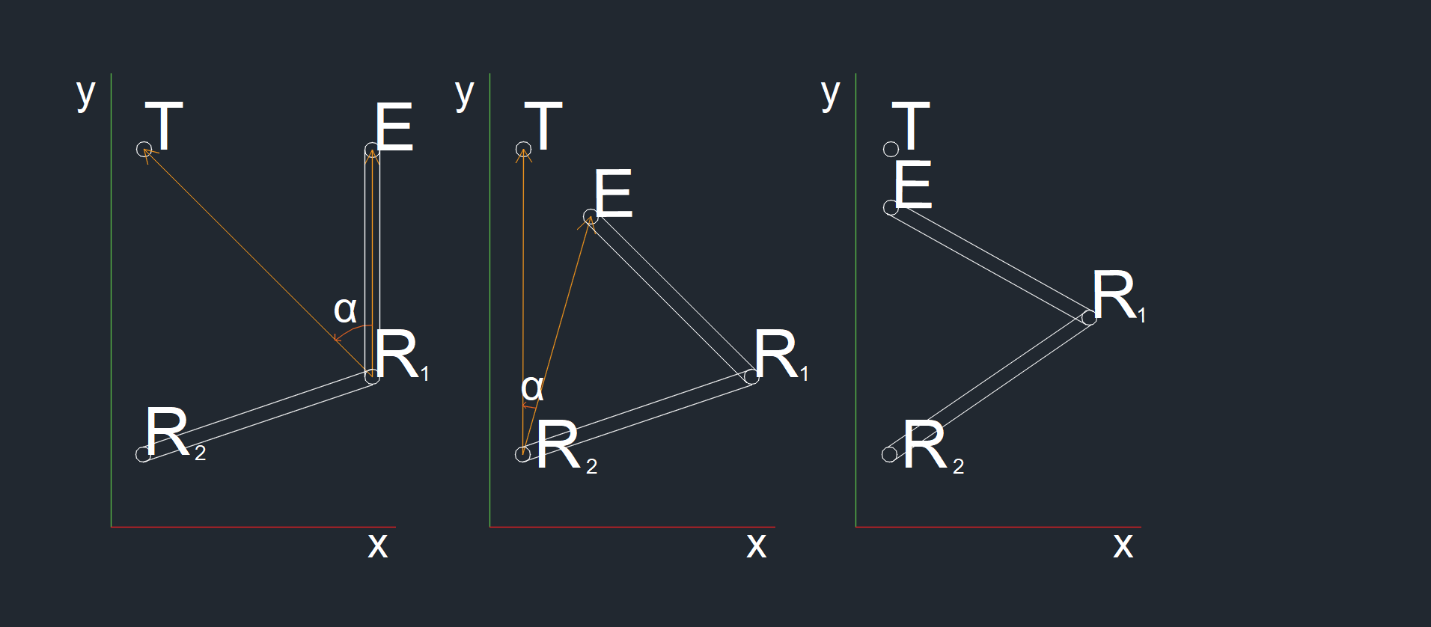
\includegraphics[scale=1]{IKCCD sketch.png}
\caption{Visual example of IK using CCD }
\end{figure}
Figure 1 Visual example of IK using CCD (add more creative caption)
In Figure 1, a desired position T, end-effector position E and position of the current joint R1 calculating the rotation for R1 is achieved by calculating the dot product R1 T⋅R1 E and the cross product R1 T×R1 E, in both cases the vectors should be normalised. Using inverse cosine, it is possible to get the angle between the two vectors, and the cross product is used to show the direction in which the root needs to be rotated. In 2D the direction of the cross product is used, however in 3D the normalised cross product vector is multiplied by the angle between the two vectors providing three new angles, for each of the three axes respectively. Those angles are directly added to the current rotation of the root joint. This process is repeated for each joint in the list.

One addition to the algorithm is the implementation of a restriction vector. The restriction is a unit vector (for example [0,0,1]), when multiplied by the new rotation vector it effectively removes any rotation from two of the axes, allowing rotation to happen only around one. This allows for more realistic movement by not allowing joints to rotate in unnatural ways.
 \begin{figure}[h]
 \centering
 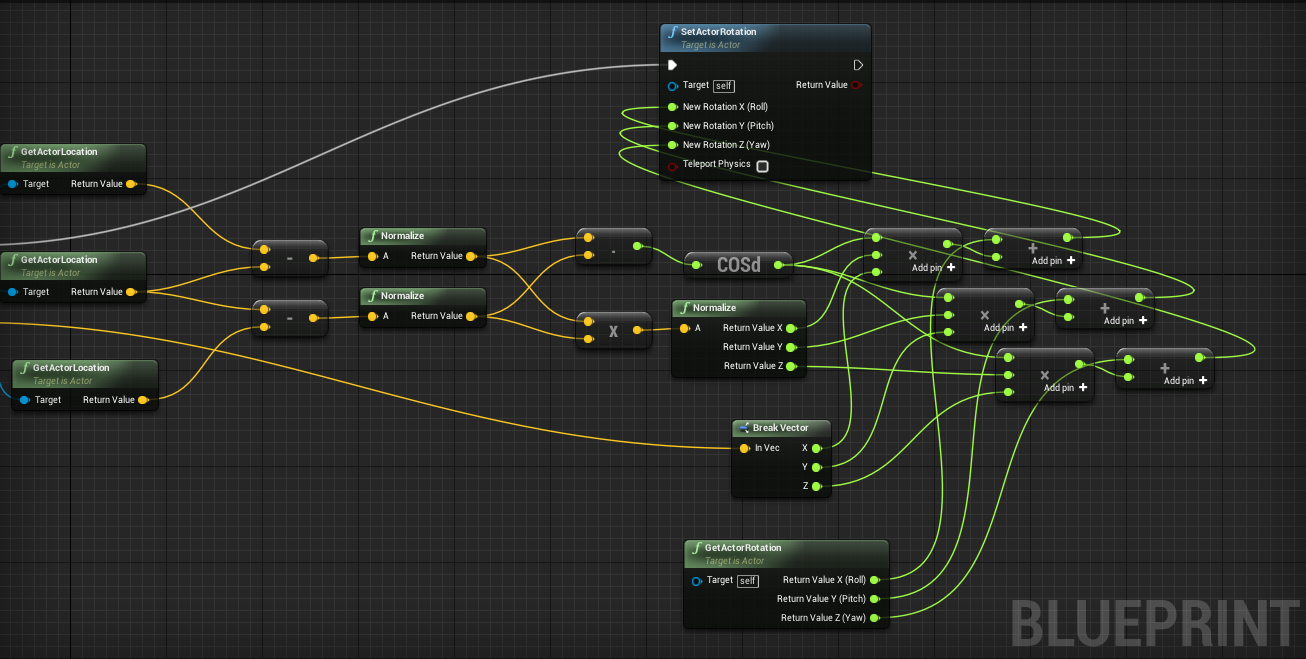
\includegraphics[scale=1]{CCDBlueprint.png}
 \caption{Blueprint that changes the rotation of object to position the end-effector closest to the desired position}
 \end{figure}
 
Figure 2 Blueprint that changes the rotation of object to position the end-effector closest to the desired position.
Because Unreal engine does not allow for easy manipulation of dedicated bone structures in real time a hierarchical joint system was used instead. Each joint share a parent child relationship with other joints in the chain, any changes made to the transform of a parent joint affects all of its children.


[1] K. W. Chin, B. R. von Konsky and A. Marriott, “Closed-form and generalized inverse kinematics solutions for the analysis of human motion,” Int. Conf. IEEE Eng. Med. Bio. Soc. 5, 1911–1914 (1997).
[2] L.-C. T. Wang and C. C. Chen, “A combined optimization method for solving the inverse kinematics problems of mechanical manipulators,” IEEE Trans. Robot. Autom. 7, 489– 499 (1991).



\section{Conclusion}


\end{document}